\documentclass[11pt]{article}
\usepackage[utf8]{inputenc}
\usepackage[T1]{fontenc}
\usepackage[francais]{babel}
\usepackage[francais]{layout}
\selectlanguage{french}


% NE PAS CHANGER !!
\ifx \public \undefined \def\public{etudiants} \fi
\usepackage[\public]{tps}

% Numéro du TP
\newcommand{\numtd}{02}
% Titre du TP
\newcommand{\titretd}{Linux~:~Utilisation distante}

\graphicspath{{imgs/}}

\begin{document}
	
\entete{\numtd}{\titretd}
 
\begin{introduction}
Ce TP est primordial car, la plupart du temps, vous utiliserez les machines à distance. Il est donc capital que vous maîtrisiez l'utilisation d'OpenSSH.
\end{introduction}

\section{Secure Shell}

Dans cette première partie, nous allons réviser les commandes de connexion à distance via SSH. Vous pourrez à titre
informatif, et/ou culturel, chercher l’équivalent de chaque commande sous MacOS et/ou Windows. OpenSSH est un outil de 
connexion à distance composé d’un client (<<ssh>> sous unix, <<putty>> sous windows, ...) et d’un serveur (<<sshd>> sous Linux).
Les fichiers de configuration d'OpenSSH se trouvent dans le repertoire <</etc/ssh/>>. Les fichiers de personnalisation du 
client se trouvent dans le homedir de l’utilisateur, dans le répertoire <<.ssh/>>.\\

Après vous être documenté sur internet, expliquer rapidement comment fonctionne la connexion d'un client SSH sur un serveur. Pourquoi peut-on dire que ce protocole est sécurisé ?

\begin{solution}
\begin{enumerate}
 \item Le client se connecte sur le serveur et ils conviennent d'un protocole de chiffrage à utiliser ;
 \item le serveur donne sa clé publique au client ;
 \item le client génère une chaine de caractère aléatoire (256bits) ;
 \item le client chiffre la chaine avec la clé publique du serveur et lui envoie le résultat ;
 \item le serveur déchiffre la chaine de caractère reçue et utilise la chaine de caractère obtenue et le protocole convenu au départ pour chiffrer les paquets envoyés au client.
 \item l'utilisateur sur le client enregistre l'empreinte du serveur dans son fichier <<\textasciitilde{}/.ssh/known\_host>> afin de détecter une future interception du trafic avec ce serveur.
\end{enumerate}

Le système est considéré comme sécurisé car aucune information non publique ne transite en clair sur le réseau.

\end{solution}


\subsection{Premières utilisations}

La syntaxe de l'utilisation du client <<ssh>> est la suivante :

\begin{lstlisting}
ssh [ options ] [ login@hostname ]  [ commande ]
\end{lstlisting}

Si le fichier <<\textasciitilde{}/.ssh/known\_hosts>> existe, renommez-le :

\begin{lstlisting}
mv ~/.ssh/known_hosts{,.old}
\end{lstlisting}

Expliquez la syntaxe proposée.

\begin{solution}

Équivalent de : mv \textasciitilde{}/.ssh/known\_hosts \textasciitilde{}/.ssh/known\_hosts.old
\end{solution}

Connectez vous au serveur SSH du département. Que ce passe-t-il ? Expliquez.

\begin{solution}

ssh ssh.dptinfo.ens-cachan.fr\\

The authenticity of host 'ssh.dptinfo.ens-cachan.fr (138.231.36.60)' can't be established.

RSA key fingerprint is SHA256:K10t1eH9D2TprjQ1tJPp+h0dz08/uFQMAdPmuPsVvDg.

Are you sure you want to continue connecting (yes/no)? 

Le système demande l'autorisation d'enregistrer l'empreinte de la clé publique du serveur.

\end{solution}

% Editer le fichier \textasciitilde{}/.ssh/known\_hosts et changer le dernier caractère de l'empreinte de la clé de SSH.

Exécuter la commande suivante :

\begin{verbatim}
sed 's/.\{5\}$/aaaaa/' ~/.ssh/known_hosts
\end{verbatim}

Se re-connecter au serveur. Que se passe-t-il ? Pourquoi ?

\begin{solution}

@@@@@@@@@@@@@@@@@@@@@@@@@@@@@@@@@@@@@@@@@@

@ WARNING: REMOTE HOST IDENTIFICATION HAS CHANGED! @

@@@@@@@@@@@@@@@@@@@@@@@@@@@@@@@@@@@@@@@@@@

IT IS POSSIBLE THAT SOMEONE IS DOING SOMETHING NASTY!

Someone could be eavesdropping on you right now (man-in-the-middle attack)!

It is also possible that a host key has just been changed.

The fingerprint for the RSA key sent by the remote host is

SHA256:K10t1eH9D2TprjQ1tJPp+h0dz08/uFQMAdPmuPsVvDg.

Please contact your system administrator.

Add correct host key in /users/fhh/.ssh/known\_hosts to get rid of this message.

Offending RSA key in /users/fhh/.ssh/known\_hosts:1

RSA host key for ssh.dptinfo.ens-cachan.fr has changed and you have requested strict checking.

Host key verification failed.
\end{solution}

Utiliser <<ssh-keygen>> pour solutionner ce problème.

\begin{solution}

ssh-keygen -R ssh.dptinfo.ens-cachan.fr
\end{solution}

\subsection{Génération d’une clef asymétrique}

\textbf{NB : } Vous verrez en détail le fonctionnement du chiffrage par clé dans le cours de crypto du second semestre.\\

OpenSSH est une implémentation du protocole SSH. Cette implémentation est open source et est libre sous Linux. Elle utilise la commande <<ssh-keygen>> pour générer
les clefs asymétriques. Utiliser la commande <<man>> pour trouver comment fonctionne la génération de clef.

Vous verrez qu’il vous est demandé, à la fin de la génération de la clef, une <<passphrase>>. La passphrase est un secret 
qui sera utilisée avec un cryptosystème symétrique.

\begin{itemize}
 \item Générez deux clefs asymétriques, l’une avec une passphrase, l’autre sans, respectivement dans les fichiers <<unsecure>> et 
<<secure>> de votre répertoire de configuration de <<SSH>>.
 \item Identifiez la partie publique et la partie privée du secret asymétrique en regardant le contenu des fichiers.
 \item Déterminez quelle partie de la clef est chiffrée. A quoi sert-il de chiffrer cette partie de la clef asymétrique ?
 \item Pourquoi pas les deux parties ?
 \item Que se passe-t-il si vous perdez la passphrase ?
\end{itemize}

\begin{solution}
\begin{itemize}
 \item <<ssh-keygen -f unsecure -C "Unsecure key" -N "">> et <<ssh-keygen -f secure -C "Secure Key" -N "">>
 \item partie publique = <<fichier.pub>> 
 \item partie protégée = <<secure>>, c'est la clé privée, la seule partie importante, qui est protégée par un mot de passe
 \item si la partie publique était chiffrée, elle ne pourrait pas être lue par les utilisateurs qui veulent l'utiliser
 \item la clé privée n'est plus utilisable
\end{itemize}
\end{solution}

\subsection{Authentification par clés}

Une façon de voir le cryptosystème asymétrique est d'imaginer que la partie publique de la clé est une serrure et que la
partie privée est la clé de cette serrure.

La mise en place de l'authentification par clés consiste à déposer, sur votre compte, dans votre répertoire <<.ssh/>>, à 
l’intérieur du fichier <<authorized\_keys>>, la partie publique de la clé (la serrure).

Nous préciserons ensuite au programme ssh quelle clé utiliser pour déverrouiller la serrure. L'accès à la clé est protégée
ou non par mot de passe.


\begin{itemize}
 \item Déployez vos clés publiques (générées précédement) dans votre homedir (en une seule commande) ;
\begin{solution}

cat unsecure.pub secure.pub $>>$ ~/.ssh/authorized\_keys
\end{solution}
 \item votre home étant distribué, essayez d'accéder au serveur ssh du département (SSH, ssh.dptinfo.ens-cachan.fr). Analysez ce qui se passe et corrigez la commande en cas de besoin.
\begin{solution}

ssh ssh.dptinfo.ens-cachan.fr\\

Le système demande mon mot de passe car les clés ne sont pas utilisées. L'option '-i' permet de spécifier la clé à utiliser\\

Connexion sans mot de passe :\\
ssh -i unsecure ssh.dptinfo.ens-cachan.fr\\

Connexion avec mot de passe de la clé :\\
ssh -i secure ssh.dptinfo.ens-cachan.fr

\end{solution}

 \item que fait la commande <<ssh-keygen -l -f unsecure>> ? et <<ssh-keygen -l -f unsecure.pub>> ? A quoi sert cette sortie ?

\begin{solution}

Affiche l'empreinte de la clé publique et privée. Cela permet de s'assurer qu'elle ne change pas au cours du temps.
\end{solution}
\end{itemize}

\subsection{Personnalisation de ssh}

Il est possible de modifier un certain nombre de paramètres de fonctionnement d'OpenSSH via le fichier <<\textasciitilde{}/.ssh/config>>.

La page de manuel de <<ssh\_config>> donnne une liste des options disponibles.

Générer un fichier de configuration permettant de se connecter au serveur SSH en utilisant l'alias <<secure>> pour utiliser la clé protégée par mot de passe et l'alias <<unsecure>> pour utiliser la clé non protégée. Tester ces configurations.

\begin{solution}

Host secure

Hostname ssh.dptinfo.ens-cachan.fr

IdentityFile \textasciitilde{}/.ssh/secure
\\

Host unsecure

Hostname ssh.dptinfo.ens-cachan.fr

IdentityFile \textasciitilde{}/.ssh/unsecure

\end{solution}

Tester la configuration .

\begin{solution}

ssh secure

ssh unsecure
\end{solution}

\subsection{Utilisation d'un porte clés}

Il est possible de gérer les clefs OpenSSH asymétriques avec un porte clef nommé <<ssh-agent>>. Ce dernier maintient les clefs en mémoire pour éviter de devoir les recharger et éviter la resaisie de la <<passphrase>>.

Quelles sont le dés/avantages de charger une clef en mémoire ?

Lancez l’agent et exportez les variables dans votre environnement. Trouvez comment ajouter une clef au porte clef. Utilisez le porte clef pour faire une connection SSH.

\begin{solution}

Possibilité d'être attaqué par un programme mal veillant, risque d'utilisation au par un utilisateur mal intentionné (exemple du coffre fort resté ouvert chez un bijoutier).

ssh-agent /bin/bash

ssh-add \textasciitilde{}/.ssh/secure

ssh secure

\end{solution}

\subsection{Différents modes de connexions}

Vous verrez en détail en deuxième année le fonctionnement du réseau dans le cours <<réseaux>>.
En attendant, imaginez une machine connectée au réseau comme un gros bloc de 65535 prises. 
Ces prises sont appelées en terminologie réseau, des ports. 
Un programme pouvant être accédé par le réseau utilise une prise. 
On dit qu'il <<écoute>> sur un port. 
Sauf cas particuliers, un port ne peut-être utilisé que par un programme à la fois. 
Les 1024 premiers ports sont réservés pour le système.
Vous pouvez utiliser les autres ports.
Un certain nombre de ports sont réservés pour des services particuliers, par exemple, le port 22 est réservé pour SSH, le port 80 est réservé pour le protocole http, le port 443 l'est pour le protocole https, etc... 
Lorsque nous utiliserons des ports pour les redirections de ports, ils devront donc <<être libre>>, c'est à dire qu'aucun programme ne les utilisera déjà, et non réservés, donc supérieurs à 1024.\\

Les techniques évoquées ci dessous vous permettront de vous connecter depuis l'extérieur sur les machines de la salle 411 ou plus généralement de vous connecter sur un réseau depuis un autre au travers d'une machine accessible en SSH.

\subsubsection{Connexion par rebond}

Se connecter à une machine située dans un réseau local peut s'illustrer par la figure~\ref{pivot_simple} page~\pageref{pivot_simple} :
\begin{enumerate}
 \item le poste <<Client 1>> se connecte à <<Passerelle SSH>> ;
 \item depuis le terminal ouvert sur <<Passerelle SSH>>, l'utilisateur ouvre une connexion sur <<Serveur cible>>.
\end{enumerate}

\begin{figure}[h]
 \centering
 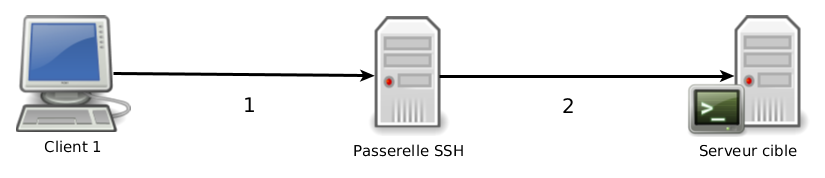
\includegraphics[width=15cm]{pivotA}
 \caption{\label{pivot_simple}Sans pivot}
\end{figure}

La machine <<Serveur cible>> n'est pas forcément accessible depuis l'extérieur.

Cette méthode ne permet pas d'exporter les applications graphiques (via l'option '-X') ou d'effectuer des copies de fichiers directement sur le serveur cible.

Essayez de vous connecter en utilisant cette méthode sur la machine de vos voisins en passant par la passerelle SSH du département.

\begin{solution}

ssh ssh.dptinfo

ssh XX.dptinfo

\end{solution}

\subsubsection{Re direction de port}

La redirection de port permet de connecter le port X d'une machine distante sur le port Y de la machine locale au travers d'une tierce machine comme l'illustre la figure~\ref{portredir} page~\pageref{portredir}. Dans ce cas :

\begin{enumerate}
 \item le poste <<Client 1>> se connecte à <<Passerelle SSH>> pour lui demander de créer un tunnel redirigeant le port X du serveur cible sur le port Y de la machine locale ;
 \item la passerelle SSH assure la mise en place de ce tunnel qui restera actif tant que la connexion restera ouverte ;
 \item à l'aide d'un autre terminal, le poste client se connecte sur l'entrée du tunnel qui redirige le trafic directement sur le port du serveur cible.
\end{enumerate}

\begin{figure}[h]
 \centering
 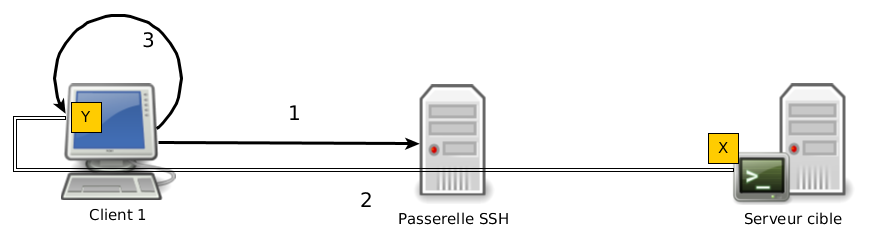
\includegraphics[width=15cm]{pivot_redirection_de_port}
 \caption{\label{portredir}Redirection de ports}
\end{figure}

\noindent \textbf{NB : } En simple utilisateur, le port Y doit être un port non privilégié (donc suppérieur à 1024).\\

L'exemple suivant redirige le port ssh (22) de la machine 22.dptinfo.ens-cachan.fr sur le port 2222 de la machine locale au travers du serveur SSH ssh.dptinfo.ens-cachan.fr :

\begin{lstlisting}
 ssh -L 2222:22.dptinfo.ens-cachan.fr:22 login@ssh.dptinfo.ens-cachan.fr
\end{lstlisting}

Dans un second terminal, il est alors possible de se connecter sur la machine 22 en empruntant le tunnel 

\begin{lstlisting}
 ssh -p 2222 login@localhost
\end{lstlisting}

Connectez vous sur la machine de votre voisin en utilisant une redirection de port SSH sur le port 1000 puis le port 2000. Que ce passe-t-il ?

Utiliser la redirection précédente pour vous connecter sur votre machine.

\begin{solution}

ssh -L 2222:22.dptinfo.ens-cachan.fr:22 login@ssh.dptinfo.ens-cachan.fr

ssh -L 2223:21.dptinfo.ens-cachan.fr:22 localhost -p 2222

\end{solution}

\subsubsection{Le pivot}

La méthode du pivot, illustrée figure~\ref{pivot} page~\pageref{pivot}, permet d'accéder à une machine au travers d'une ou plusieurs autres de manière quasi transparente.\\

\begin{figure}[h]
 \centering
 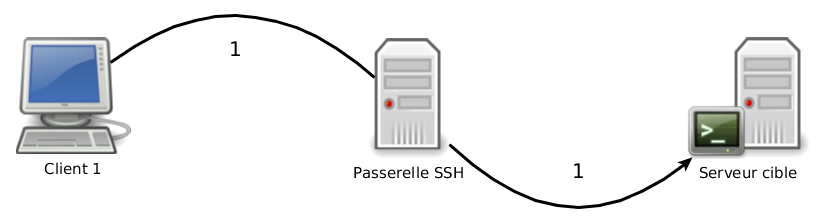
\includegraphics[width=15cm]{pivot}
 \caption{\label{pivot}Méthode du pivot}
\end{figure}

Au contraire de la connexion par rebond, l'utilisation de la passerelle est transparente pour l'utilisateur. La connexion étant redirigée à la manière de la redirection de port, l'export X fonctionne.

\noindent\textbf{\underline{Via le fichier de configuration de ssh}}\\

L'option <<ProxyCommand>>, ajoutée à la définition d'un alias dans le fichier de personnalisation du client ssh, permet de spécifier la machine utilisée comme pivot.

\begin{lstlisting}
Host <alias_machine>
Hostname <machine.cible>
User <login_sur_machine cible>
ProxyCommand ssh <login>@<machine.ssh.pivot> -W %h:%p
\end{lstlisting}

où :
\begin{itemize}
 \item{<alias\_machine>} le nom qui sera utilisé pour appeler cette configuration ;
 \item{<machine.cible>} machine sur laquelle nous souhaitons arriver ;
 \item{<login\_sur\_machine\_cible>} login à utiliser sur la machine cible, si non précisé, login courant utilisé ;
 \item{<login>@<machine.ssh.pivot>} paramètres de connexion sur la machine pivot.\\
\end{itemize}

Consulter la page de manuel de <<ssh\_config>> pour vous documenter sur l'option <<-W>>.

Configurez un alias vous permettant de vous connecter sur votre machine au travers du serveur SSH du département d'informatique. 
Ajouter l'utilisation de la clé SSH <<secure>> précédement générée.\\

\textbf{NB :} Vous pouvez utiliser les alias lors de la création de vos alias.\\

\noindent\textbf{\underline{Via les nouvelles fonctionnalités d'ssh}}\\

Nous avons compilé, lors du TP précédent, une version récente d'OpenSSH qui offre une nouvelle option '-J' qui permet de spécifier un pivot lors d'une connexion.

La configuration précédente peut alors s'écrire 

\begin{lstlisting}
ssh -J <login>@<machine.ssh.pivot> <login_sur_machine_cible>@<machine.cible>
\end{lstlisting}

Testez la connexion à la machine de votre voisin au travers du serveur SSH du département.

\textbf{NB :} Vous pouvez également utiliser l'option <<ProxyJump $<$login$>$@$<$machine.ssh.pivot$>$>> dans votre fichier de configuration. Cette option à été introduite dans OpenSSH 7.3.

\subsection{Proxy SOCKS}

Vous pouvez utiliser un serveur SSH comme serveur proxy (serveur mandataire) comme illustré sur la figure~\ref{socks} page~\pageref{socks}, c'est a dire que votre trafic web passera par le serveur SSH et que vous naviguerez comme si vous vous trouviez dans les murs de l'ENSC.\\

\begin{figure}[h]
 \centering
 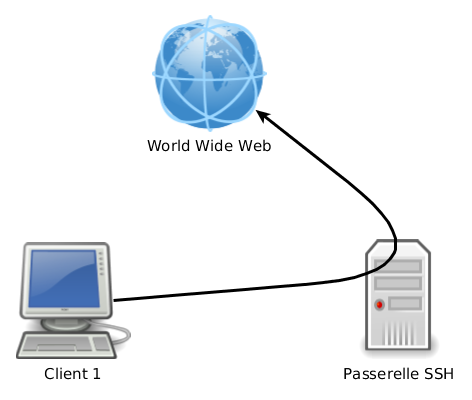
\includegraphics[width=9cm]{socks}
 \caption{\label{socks}Proxy SOCKS}
\end{figure}

\begin{itemize}
 \item Cherchez sur Google, avec firefox, un site affichant votre adresse IP ;
 \item dans un terminal utiliser l'option <<-D $<$port\_non\_reservé$>$>> pour créer un proxy local (consulter le manuel de ssh pour voir comment utiliser l'option) ;
 \item configurer votre navigateur internet pour utiliser votre proxy local ; avec Firefox :
 \begin{itemize}
  \item rendez-vous dans <<préférences>> puis <<Avancé>> (page about:preferences\#advanced) et selectionnez l'onglet <<réseaux>> ;
  \item configurez le mode de connexion au réseau en cliquant sur <<configuration>>
  \item dans la nouvelle fenêtre activez <<Configuration manuelle>> et renseignez les champs <<SOCKS Host>> = localhost et <<Port>> = $<$port\_non\_reservé$>$ spécifié précédement.
  \item validez par <<Ok>>
 \end{itemize}
 \item rafraichir la page du site affichant votre IP. Que constatez vous ?
 \item Fermez la connexion ssh ouverte puis rafraichissez la page web affichant votre IP. Que ce passe-t-il ? Pourquoi ?
\end{itemize}

\section{Multiplexeur de terminal}

L'outil <<tmux>> vous permet d'ouvrir plusieurs instances du shell dans un même terminal et donc via SSH par exemple.

\begin{itemize}
 \item Lancez <<tmux>> dans un terminal. 
 \item Lancez la commande <<top>>.
 \item Ouvrir une nouvelle instance du terminal via <<Ctrl+b>> (pour signaler que nous envoyons la commande à <<tmux>>) puis <<c>> (pour create)
 \item Listez le contenu du répertoire courant
 \item Retourner sur le shell executant "top" via <<Ctrl+b>> puis <<p>> (previous). Utilisez <<Ctrl+b>> puis <<n>> pour l'écran suivant (next).
 \item <<Splitez>> l'écran verticalement <<Ctrl+b>> puis <<">>.
 \item <<Splitez>> l'écran horizontalement <<Ctrl+b>> puis <<\%>>.
 \item Détachez ce tmux du terminal <<Ctrl+b>> puis <<d>>.
 \item Ré attachez votre tmux au terminal <<tmux a>>.
 \item Vérifiez que <<top>> fonctionne toujours.
\end{itemize}

Le manuel de tmux et Google vous donneront toutes les astuces du fonctionnement de ce programme.

\end{document}
